\procTitle{Перспективы развития междисциплинарных геокриологических исследований на~Северо-Востоке России}
\procAuthor{Нестерова~Н.\,В., Землянскова~А.\,А., Осташов~А.\,А.}
\procEmail{nnesterova1994@gmail.com}
\procOrganization{СВНИМС ИМЗ СО РАН} \procCity{Магадан}

\makeProcTitle
\index{z@Землянскова~А.\,А.}
\index{n@Нестерова~Н.\,В.}
\index{o@Осташов~А.\,А.}

В прогнозе долгосрочного социально-экономического развития РФ на~период до 2030~г. изменения климата указаны в качестве одного из основных внешних вызовов [2].

Деградация криолитозоны, изменение мощности деятельного слоя, конфигурации таликов, типов ландшафтов и другие факторы приводят к изменению водообмена между поверхностными и подземными водами. Механизмы взаимодействия поверхностного и подземного стока, водовмещающих пород и мёрзлых отложений изменчивы в пространстве и~во~многом определяются ландшафтными характеристиками. Количественные оценки реакции мерзлоты, влияния динамики деятельного слоя на связь поверхностных и подземных вод и~формирование речного стока в будущем остаются неопределёнными вследствие нелинейного характера взаимодействий климата и мерзлотных ландшафтов [3--6].

Одновременно усиливается антропогенное воздействие, связанное с индустриальным и~инфраструктурным освоением северных территорий, в том числе с разработкой и обустройством месторождений полезных ископаемых, строительством дорог, линий электропередачи и других линейных сооружений, промышленных объектов и населённых пунктов, строительством гидротехнических сооружений и др. [1]. Все эти работы в той или иной мере оказывают влияние на естественные ландшафты и протекающие в них процессы.

Поэтому научное изучение происходящих изменений в системе водообмена Северо-Востока, их прогноз на ближайшее будущее остаётся насущной задачей научного обеспечения развития территории Северо-Востока. Несмотря на то что водообменные процессы являются основой функционирования криолитозоны, различные науки о Земле традиционно фокусируются на отдельных компонентах единой природной системы. Сложность рассматриваемых процессов, объединённых потоками воды и тепла, обусловливает необходимость применения междисциплинарного научного подхода.

В настоящей работе коллективом авторов предлагается видение организации комплексных исследований в целях оценки и прогноза изменения условий водообмена подземных и~поверхностных вод в естественных и нарушенных условиях в бассейнах рек криолитозоны Северо-Востока, в том числе для решения прикладных задач, на основе методов мерзлотоведения, гидрологии, гидрогеологии, ландшафтоведения и геофизики с применением дистанционного зондирования Земли и полевых исследований, объединённых методами математического моделирования (см. рисунок).

\begin{figure}[h!]
%\begin{changemargin}{-1.25cm}{0cm}
  \begin{center}
    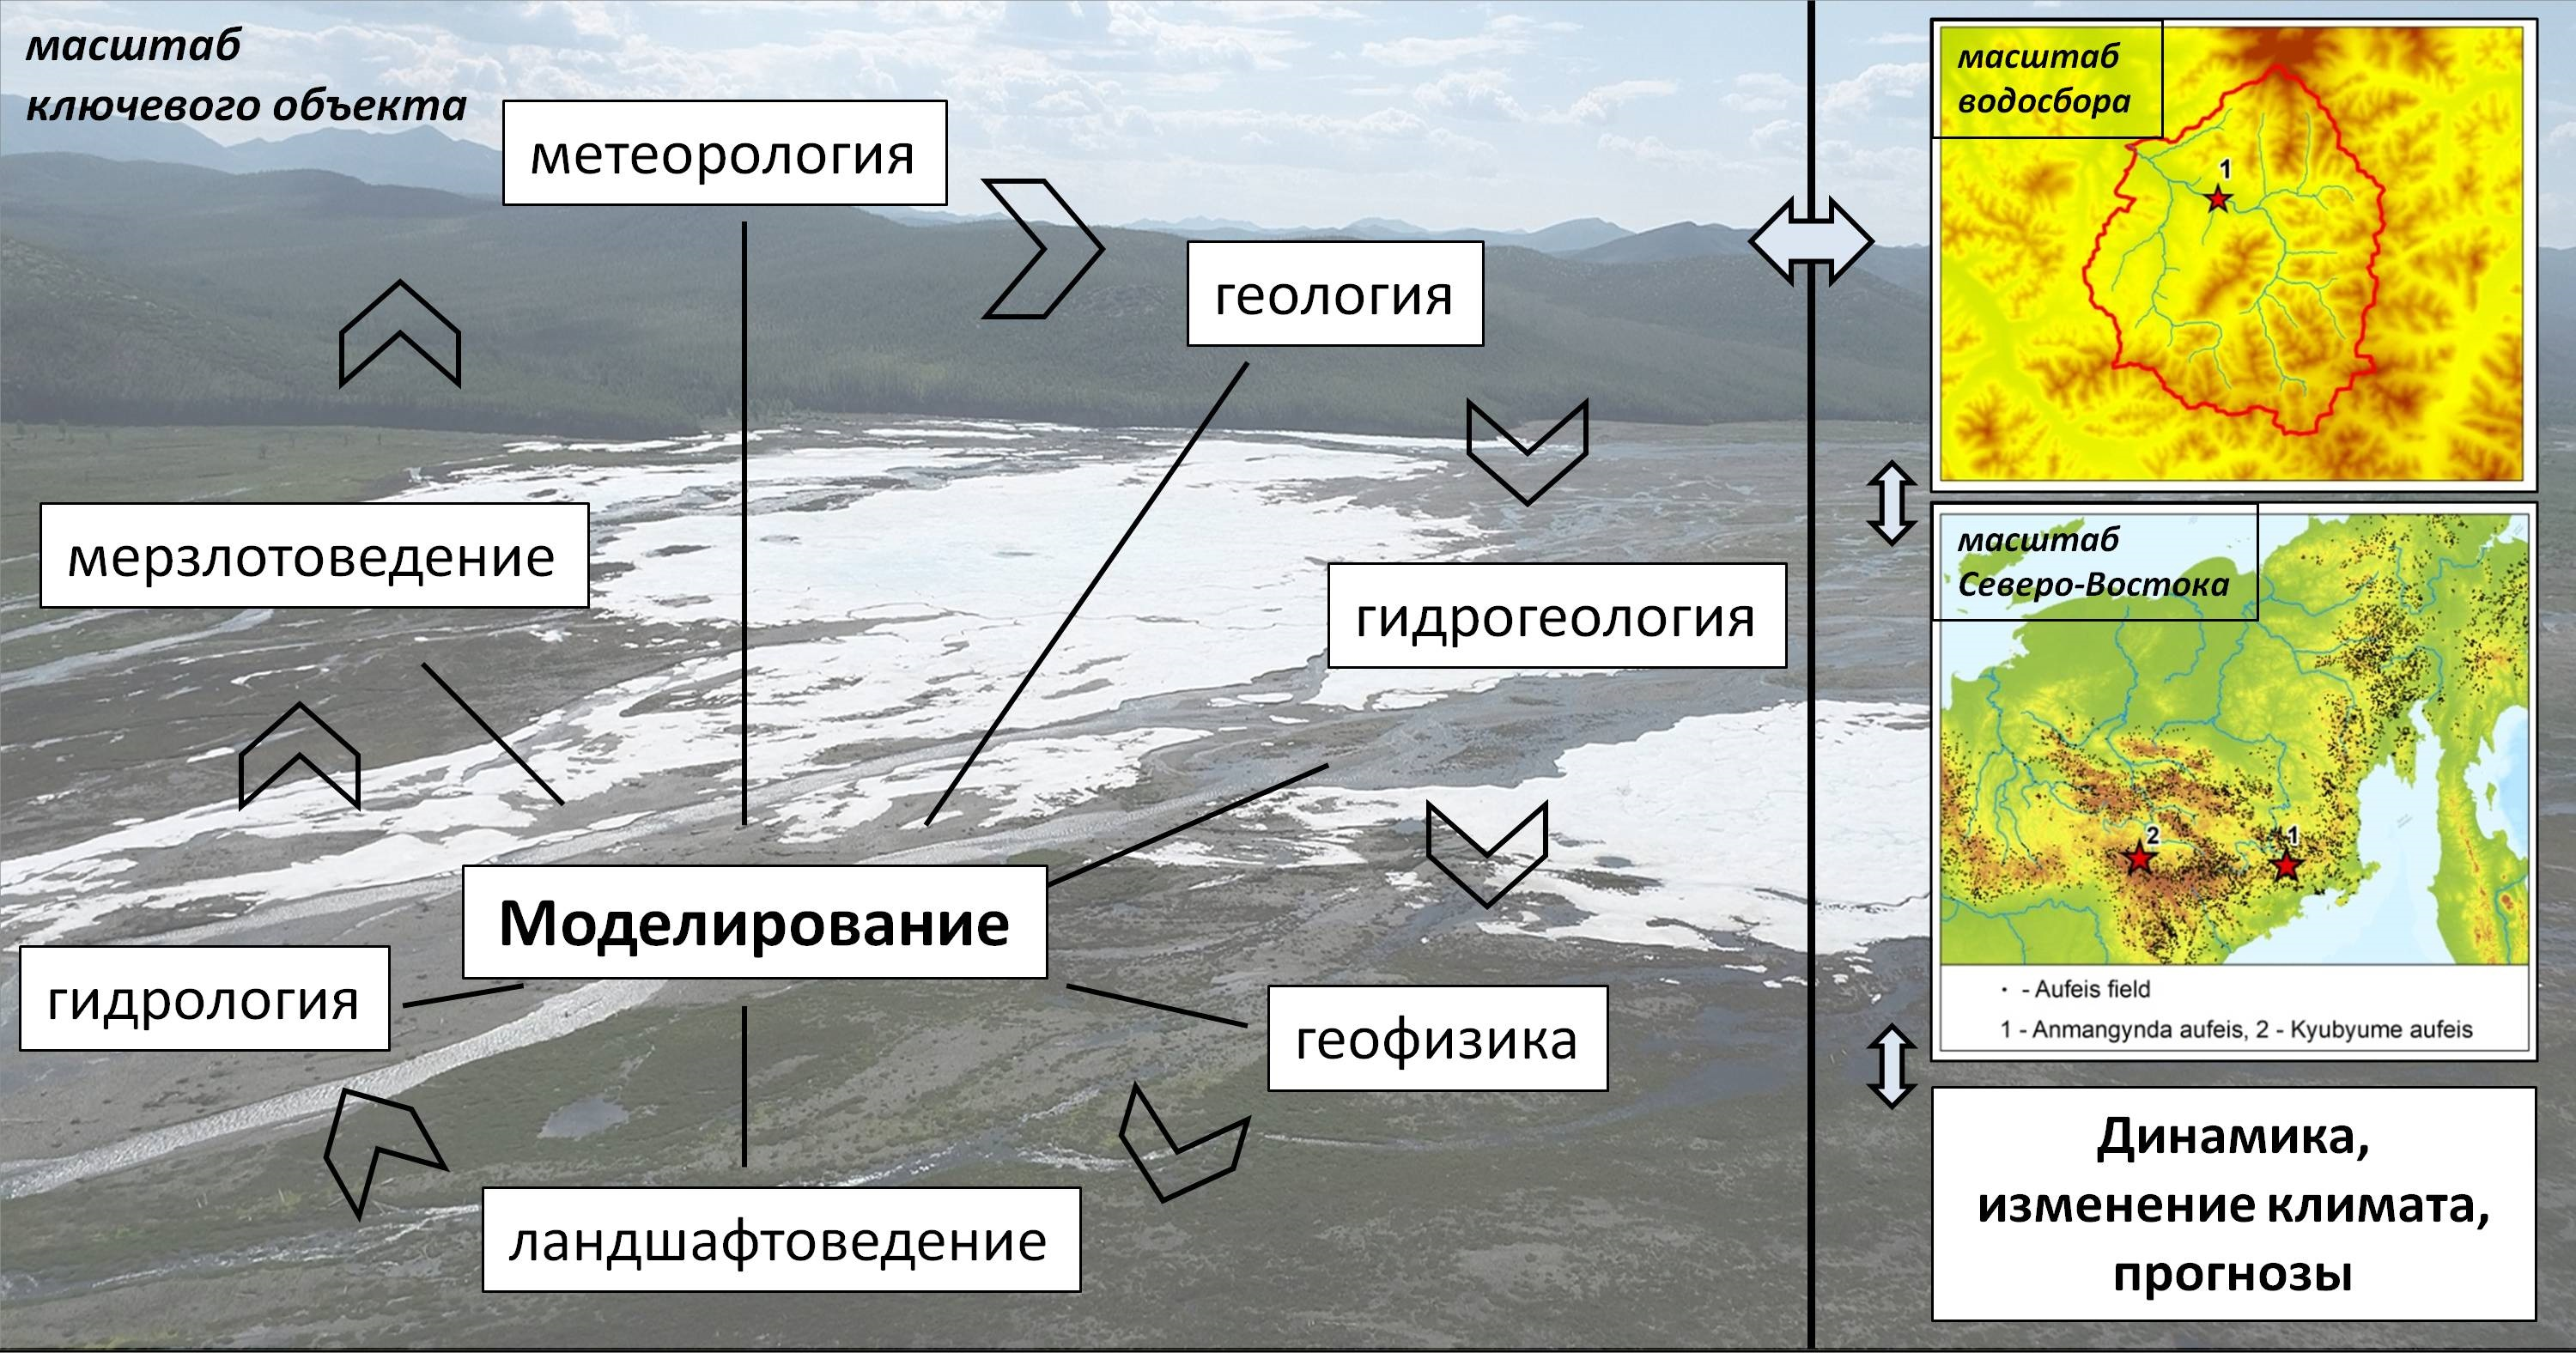
\includegraphics[width=1\textwidth]{authors/nesterova-2-fig-1.jpg}
  \end{center}
%\end{changemargin}
  \caption*{\textbf{Схема потенциальных исследований}}
  \label{fig:nesterova-1-fig-1}
\end{figure}


\textbf{Потенциальные объекты исследования}

На территории Северо-Востока России (Магаданская область) расположены уникальные научные стационары и природные объекты, на которых мониторинг гидрологических и криогенных процессов, типичных для всего региона, а также значительных по площади горных территорий Сибири и~Северо-Востока, производился на протяжении десятков лет. Среди них~--- Колымская водно-балансовая станция (КВБС) (пос.~Стоковое), функционировавшая в период 1948--1997~гг., а также стационар Анмангындинской наледи (25~км от~пос.~Усть-Омчуг), на котором проводились наблюдения с~1962 до конца 1990-х~гг. Таких стационаров с длительным рядом наблюдений не существует ни в одной северной стране мира.

Также следует выделить потенциальные объекты исследования: наледь Кюбюме, расположенную в бассейне р. Кюбюме в 180~км к юго-западу от~пос.~Усть-Нера, на которой Северо-Восточным федеральным университетом имени М.~К.~Аммосова проводятся Школы-экспедиции, а также стационар Института биологических проблем севера в Чаунской губе. Все упомянутые объекты являются репрезентативными для территории Северо-Востока России и имеют основу для проведения междисциплинарных исследований.

\textbf{Методы и предполагаемые результаты}

Под междисциплинарностью исследования предполагается использование целого комплекса различных методов, среди которых:
\begin{itemize}[noitemsep]\vspace{-8pt}
  \item методы дистанционного зондирования и полевые описания мерзлотных ландшафтов;
  \item геофизические методы исследований и бурение скважин;
  \item режимные гидрометеорологические наблюдения, гидрологический, гидрогеологический и геокриологический мониторинг;
  \item геохимические и изотопные методы исследований водообмена и качества природных вод (речных и подземных, а также атмосферных осадков);
  \item математическое моделирование пространственно-временной динамики толщ мёрзлых и талых пород, её влияния на процессы формирования речного стока и интенсивность водообмена подземных и поверхностных вод.
\end{itemize}
 \vspace{-8pt}
Научная новизна исследований заключается в следующем.

Впервые за последние 30~лет на Северо-Востоке России предлагается организовать комплексный мониторинг состояния мерзлоты, гидрогеологических условий и процессов формирования стока на нескольких ключевых участках. Репрезентативность выбранных ключевых участков позволит перенести результаты исследований на региональный уровень, а~разработанные подходы к решению поставленной задачи будут актуальны и для других регионов криолитозоны.
\clearpage
Вновь организованные режимные наблюдения на опорном наледном полигоне позволят изучить динамику наледеобразующих источников и осуществить расчёт динамических запасов подземных вод. Геофизические и гидрогеологические данные будут использованы для установления связи между типами и структурой гидрографической сети и местоположением подрусловых таликов. Это даст возможность оценить интенсивность и трансформацию водообменных процессов при изменении природной среды и климата.

Впервые на основе данных мониторинга, изотопной геохимии и разработанной модели водообмена предполагается дать количественные оценки доли подземного питания в стоке рек в различные фазы водного режима Северо-Востока.

Впервые на основе данных дистанционного зондирования предлагается составить <<Атлас мерзлотных ландшафтов>>, включая ландшафты, нарушенные в результате деятельности золотодобывающих компаний. С учётом опубликованных и вновь полученных данных атлас позволит систематизировать прогнозируемые изменения водообмена в различных типах ландшафтов в зависимости от реакции мёрзлых толщ и таликов на климатические изменения, а также оценить степень преобразования системы водообмена в~пределах антропогенно-нарушенных участков, а также их вклад в~изменение гидрологического и~экологического режима рек Северо-Востока.

Также для региона Северо-Востока предлагается разработать прогноз изменений режима и геохимического состава природных вод как следствие трансформации структуры водообмена в результате потепления климата и~деятельности человека.

Возможность реализации перечисленных перспектив развития научных стационаров на~территории криолитозоны Северо-Востока России определяется следующими факторами:
\begin{itemize}[noitemsep]\vspace{-6pt}
\item наличием данных непрерывных долгосрочных наблюдений за состоянием мерзлоты, гидрогеологическими условиями и стоком рек на~выбранных ключевых участках в~исторический период, что позволит проследить динамику трансформаций характеристик мерзлоты, гидрогеологических условий и стока и связать их с изменениями климата;\vspace{2pt}
\item традиционными методами исследования состояния талых и мёрзлых зон (мониторинг, ландшафтная индикация, бурение), которые будут дополнены детальными геофизическими съёмками, методами изотопной геохимии и гидрохимии, автоматизированными наблюдениями с высоким временным разрешением и математическим моделированием;\vspace{2pt}
\item использованием методов моделирования, в явном виде учитывающих динамику деятельного слоя и его переменных состояний в гидрологических расчётах. Разработка новых алгоритмов и параметризации, описывающих механизмы связи подземных и~поверхностных вод будет производиться совместно с геокриологами на основе данных мониторинга;\vspace{2pt}
\item наличием инфраструктуры и человеческих ресурсов для организации полноценного комплексного мониторинга объектов исследования;\vspace{2pt}
\item междисциплинарным составом и опытом участников;\vspace{2pt}
\item хаинтересованностью региональных и муниципальных органов власти и населения.
\end{itemize}
 \vspace{-6pt}

Перспективы могут быть реализованы только на основе привлечения молодых научных кадров, что обусловливает необходимость тесного взаимодействия исследовательских институтов и университетов.

Решение поставленной задачи и обобщение результатов возможно только на региональном уровне с учётом особенностей климата, геологического строения, рельефа, геокриологических характеристик, ландшафтов. В~значительной степени оно зависит от наличия полевых данных совместных наблюдений за динамикой состояния мерзлоты, гидрогеологическими условиями на водосборах и стоком рек, позволяющих не только выявить механизмы их взаимодействия, но и проследить динамику в исторической перспективе, обосновать прогноз изменений в будущем.

\textit{Исследования проводятся при поддержке РФФИ~--- проекты №~20-05-00666\,А, 19-35-90090, 19-55-80028 и РГО проект <<Атлас гигантских наледей-тарынов Северо-Востока России>>.}

\begin{thebibliography}{99}
\bibitem{}\BibAuthor{Алексеевский~Н.~И., Магрицкий~Д.~В., Михайлов~В.~Н.} Антропогенные и~естественные изменения гидрологических ограничений для природопользования в дельтах рек Российской Арктики // Водное хозяйство России: проблемы, технологии, управление.~--- 2015.~--- №~1.~--- С.~14--31.
\bibitem{}Оценочный доклад об изменениях климата и их последствиях на территории Российской Федерации [Электронный ресурс].~--- М.~: Росгидромет, 2008.~--- URL:~http://climate2008.igce.ru (дата обращения: 15.10.2020).
\bibitem{}\BibAuthor{Романовский~Н.~Н., Булдович~С.~Н., Типенко~Г.~С.} Оценка влияния климатических изменений на поверхностный сток с помощью моделирования теплового взаимодействия многолетне\-мёрзлых пород и подземных вод (на примере верхней части водосборного бассейна р.~Лены)~// Криосфера Земли.~--- 2009.~--- Т.~13, №~1.~--- С.~55--64.
\bibitem{}\BibAuthor{Шикломанов~И.~А., Георгиевский~В.~Ю.} Влияние изменений климата на гидрологический режим и водные ресурсы рек России~// Гидрологические последствия изменения климата.~--- Новосибирск, 2007.~--- С.~192--204.
\bibitem{}\BibAuthor{Makarieva~O., Nesterova~N., Post~D.~A., Sherstyukov~A., Lebedeva~L.} Warming temperatures are impacting the hydrometeorological regime of Russian rivers in the zone of continuous permafrost~// The Cryosphere.~--- 2019.~--- Vol.~13.~--- P.~1635--1659.~--- DOI:~10.5194/tc-13-1635-2019.
\bibitem{}\BibAuthor{Tananaev~N.~I., Makarieva~O.~M., Lebedeva~L.~S.} Trends in annual and extreme flows in the Lena River basin, Northern Eurasia // Geophys. Res. Lett.~--- 2016.~--- Vol.~43.~--- P.~10\,764--10\,772.~--- DOI:~10.1002/2016GL070796.

\end{thebibliography}
